              
                %%%%%%%%%%%%%%%%%%%%%%%%%%%%%%%%%%%%%%%%%
% Journal Article
% LaTeX Template
% Version 1.3 (9/9/13)
%
% This template has been downloaded from:
% http://www.LaTeXTemplates.com
%
% Original author:
% Frits Wenneker (http://www.howtotex.com)
%
% License:
% CC BY-NC-SA 3.0 (http://creativecommons.org/licenses/by-nc-sa/3.0/)
%
%%%%%%%%%%%%%%%%%%%%%%%%%%%%%%%%%%%%%%%%%
%----------------------------------------------------------------------------------------
%       PACKAGES AND OTHER DOCUMENT CONFIGURATIONS
%----------------------------------------------------------------------------------------
\documentclass[paper=letter, fontsize=12pt]{article}
\usepackage[english]{babel} % English language/hyphenation
\usepackage{amsmath,amsfonts,amsthm} % Math packages
\usepackage[utf8]{inputenc}
\usepackage{float}
\usepackage{lipsum} % Package to generate dummy text throughout this template
\usepackage{blindtext}
\usepackage{graphicx} 
\usepackage{caption}
\usepackage{subcaption}
\usepackage[sc]{mathpazo} % Use the Palatino font
\usepackage[T1]{fontenc} % Use 8-bit encoding that has 256 glyphs
\linespread{1.05} % Line spacing - Palatino needs more space between lines
\usepackage{microtype} % Slightly tweak font spacing for aesthetics
\usepackage[hmarginratio=1:1,top=32mm,columnsep=20pt]{geometry} % Document margins
\usepackage{multicol} % Used for the two-column layout of the document
%\usepackage[hang, small,labelfont=bf,up,textfont=it,up]{caption} % Custom captions under/above floats in tables or figures
\usepackage{booktabs} % Horizontal rules in tables
\usepackage{float} % Required for tables and figures in the multi-column environment - they need to be placed in specific locations with the [H] (e.g. \begin{table}[H])
\usepackage{hyperref} % For hyperlinks in the PDF
\usepackage{lettrine} % The lettrine is the first enlarged letter at the beginning of the text
\usepackage{paralist} % Used for the compactitem environment which makes bullet points with less space between them
\usepackage{abstract} % Allows abstract customization
\renewcommand{\abstractnamefont}{\normalfont\bfseries} % Set the "Abstract" text to bold
\renewcommand{\abstracttextfont}{\normalfont\small\itshape} % Set the abstract itself to small italic text
\usepackage{titlesec} % Allows customization of titles

\usepackage[version=4]{mhchem}  % for chemical reactions
\newcommand\reaction[1]{\begin{equation}\ce{#1}\end{equation}}
\newcommand\reactionnonumber[1]%
{\begin{equation*}\ce{#1}\end{equation*}}
\usepackage{tikz} % using TikZ pictures


\renewcommand\thesection{\Roman{section}} % Roman numerals for the sections
\renewcommand\thesubsection{\Roman{subsection}} % Roman numerals for subsections

\titleformat{\section}[block]{\large\scshape\centering}{\thesection.}{1em}{} % Change the look of the section titles
\titleformat{\subsection}[block]{\large}{\thesubsection.}{1em}{} % Change the look of the section titles
\newcommand{\horrule}[1]{\rule{\linewidth}{#1}} % Create horizontal rule command with 1 argument of height
\usepackage{fancyhdr} % Headers and footers
\pagestyle{fancy} % All pages have headers and footers
\fancyhead{} % Blank out the default header
\fancyfoot{} % Blank out the default footer

\fancyhead[C]{Otto von Guericke Universität Magdeburg $\bullet$ Summersemester 2017 $\bullet$ Process Control } % Custom header text

\fancyfoot[RO,LE]{\thepage} % Custom footer text
%----------------------------------------------------------------------------------------
%       TITLE SECTION
%----------------------------------------------------------------------------------------
\title{\vspace{-15mm}\fontsize{24pt}{10pt}\selectfont\textbf{Control of a Single Process Unit: Dynamic Model of Ammonia Synthesis Reactor}} % Article title
\author{
\large
{\textsc{Pascal Bock\footnote{contact: \href{mailto:pascal.bock@st.ovgu.de}{pascal.bock@st.ovgu.de}}, 199368 }}\\[2mm]
{\textsc{Jakob Kübler, 199197 }}\\[2mm]
{\textsc{Christian Weidele, 200329 }}\\[2mm]
%\thanks{A thank you or further information}\\ % Your name
%\normalsize \href{mailto:marco.torres.810@gmail.com}{marco.torres.810@gmail.com}\\[2mm] % Your email address
}
\date{}

%----------------------------------------------------------------------------------------
\begin{document}
\maketitle % Insert title
\thispagestyle{fancy} % All pages have headers and footers


\section{Introduction}
The aim of the course \emph{Process Control} is to control a multivariable process unit. To do so, we will follow four steps for control system design. First we will model the system (\autoref{s:modelDevelopment}) before we will analyse the model in a second step. After that we will design and implement a controller as third and fourth step. \\
Our focus lays not on developing a model, so we need a well documented multivariable model which is not to complex. With \cite{Jinasena2016} we found a good documented multivariable model of the ammonia synthesis. Other approaches of dynamic simulation of ammonia synthesis can be found in \cite{Kasiri2003} using Soave-Redlich-Kwong equation and modeling a four-bed ammonia synthesis catalytic reactor and \cite{Mancusi2009} using a three-bed ammonia synthesis catalytic reactor. In \cite{Morud1998} a model based on the Arrhenius equation for for- and backward reaction is considered. But all these are not as good documented as \cite{Jinasena2016} in which the Arrhenius equation is only used for the reverse reaction rate constant and the reaction rate for the forward reaction is based on the Gillespie-Beattie correlation.\\
Ammonia is critical for production of fertilizers and one of the most produced chemicals in the world. The production of high amounts of ammonia made the fast growing world population of the last century possible. \cite{Pattabathula2016} \\
Despite the simplicity of the model it is possible to simulate the unnstable behaviour of the system and the oscillatory behaviour of the temperature when steady state is disturbed. A controller not only for feed temperature before heat exchanger also for feed flow rate and composition of feed is recommended in \cite{Jinasena2016}. Using a simple PI-controller for temperature regulation is considered for a more complex model of ammonia synthesis in \cite{Morud1998}.


\section{Model Development} \label{s:modelDevelopment}

The model describes the Haber-Bosch process by focusing on the main reaction
\reaction{N2(g) + 3H2(g) <=>[Fe] 2NH3(g).} \label{f:reaction}
In addition to \ce{N2} and \ce{H2} Argon (\ce{Ar}) is used as an inert gas. The reactor is using an iron (\ce{Fe}) based catalyst. The same assumptions as in \cite{Jinasena2016} are holding.\\
In this chapter we will show a short derivation of the model equation we used in Matlab. We will proceed in four steps. First we will derive the mole balances. For solving these we need to develop an equation for the accumulation term and derive the energy balance in a second and third step. And in a last step we will evolve the equations for the heat exchanger.

% TikZ picture
\begin{figure}
\begin{centering}
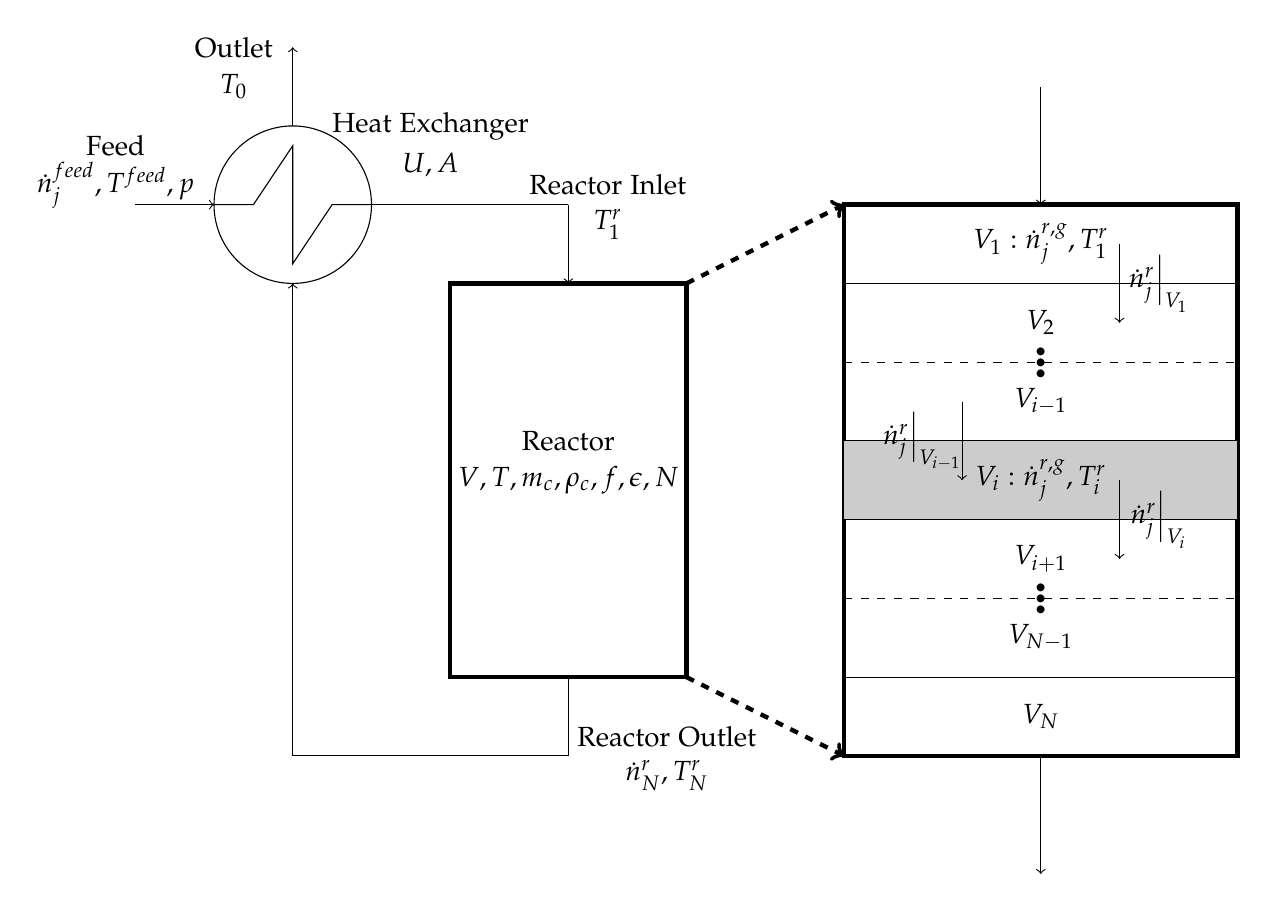
\begin{tikzpicture}

%% full flow chart
\draw (0,0) circle (1 cm); % heat exchanger
\draw [ultra thick] (5,-1) rectangle (2,-6) ;  % reactor
\draw (1,0) -- (3.5,0); % from heater to right
\draw [->] (3.5,0) -- (3.5,-1); % to reactor from above
\draw (3.5,-6) -- (3.5,-7) -- (0,-7); % from outlet of reactor to heater x-coordinate
\draw [->] (0,-7) -- (0,-1); % to heat exchanger from below
\draw [->] (-2,0) -- (-1,0); % from left to heat exchanger
\draw [->] (0,1) -- (0,2); % from heat exchanger to above
\draw (-1,0) -- (-0.5,0) -- (0,.75) -- (0,-.75) -- (0.5,0) -- (1,0); % 'curve' in heat exchanger

%%  labeling
\node at (1.75,1) {Heat Exchanger};
\node at (1.75,.5) {$U, A$};
\node at (3.5,-3) {Reactor};
\node at (3.5,-3.5) {$V,T,m_c,\rho_c,f,\epsilon,N$};
\node at (-2.25,0.75) {Feed};
\node at (-2.25,.25) {$\dot{n}^{feed}_j, T^{feed},p$};
\node at (4.75,-6.75) {Reactor Outlet};
\node at (4.75,-7.25) {$\dot{n}^r_N, T^r_N$};
\node at (4,0.25) {Reactor Inlet};
\node at (4,-0.25) {$T^r_1$};
\node at (-.75,2) {Outlet};
\node at (-.75,1.5) {$T_0$};

%% zoom on reactor
\draw [->, ultra thick, dashed] (5,-1) -- (7,0); % arrow
\draw [->, ultra thick, dashed] (5,-6) -- (7,-7); % arrow
\draw [ultra thick] (12,0) rectangle (7,-7) ; % reactor
\draw [->] (9.5,1.5) -- (9.5,0); % inlet arrow
\draw [->]  (9.5,-7) -- (9.5,-8.5); % outlet arrow
\draw (7,-1) --(12,-1); % V_1
\draw [dashed] (7,-2) --(12,-2); % dashed one up
%\draw (7,-3) --(12,-3);
%\draw (7,-4) --(12,-4);
\draw [fill=black!20] (12,-3) rectangle (7,-4); % V_i
\draw [dashed] (7,-5) --(12,-5); % dashed one down
\draw (7,-6) --(12,-6); % V_N
% labeling
\node at (9.5,-.5) {$V_1: \dot{n}^{r,g}_j, T^r_1$};
\node at (9.5,-1.5) {$V_2$};
\node at (9.5,-1.9) {\Huge $\vdots$};
\node at (9.5,-2.5) {$V_{i-1}$};
\node at (9.5,-3.5) {$V_i : \dot{n}^{r,g}_j, T^r_i$};
\node at (9.5,-4.5) {$V_{i+1}$};
\node at (9.5,-4.9) {\Huge $\vdots$};
\node at (9.5,-5.5) {$V_{N-1}$};
\node at (9.5,-6.5) {$V_N$};
% arrows inside compartments
\draw [->]  (10.5,-0.5) -- (10.5,-1.5); %first arrow
\node at (11,-1) {$\dot{n}^r_j \Big|_{V_{1}} $};
\draw [->]  (8.5,-2.5) -- (8.5,-3.5); %left arrow
\node at (8,-3) {$\dot{n}^r_j \Big|_{V_{i-1}} $};
\draw [->]  (10.5,-3.5) -- (10.5,-4.5); %right arrow
\node at (11,-4) {$\dot{n}^r_j \Big|_{V_{i}} $};

\end{tikzpicture}
\caption{Flow sheet of reactor and heat exchanger (according to \cite{Jinasena2016}) and volume compartments $V_i=\frac{V}{N}$}
\end{centering}
\end{figure}

\subsection{Molar Balance of Volume Compartment}
For a volume compartment  $V_i=\frac{V}{N}, i=\lbrace 1,2 \dots, N \rbrace$ the mole balance equation is given as
\begin{align}
\frac{d}{dt} n^r_j \Big|_{V_i}= \dot{n}^r_j\Big|_{V_{i-1}} - \dot{n}^r_j\Big|_{V_{i}} + \dot{n}^{r,g}_j\Big|_{V_{i}}. \label{f:molebalance}
\end{align}
At this, $\dot{n}^r_j\Big|_{V_{i-1}}$ is the molar stream coming from the volume compartment before, $\dot{n}^r_j\Big|_{V_{i}}$ is the molar outlet stream of $V_i$ and $\dot{n}^{r,g}_j\Big|_{V_{i}}$ describes the moles generated of species $j \in \lbrace \ce{N2}, \ce{H2}, \ce{NH3}, \ce{Ar} \rbrace$ in volume compartment $V_i$. For $i=1$ the inlet stream is the molar feed stream, this also hold for the energy balance in \autoref{s:energyBalance}. \\

\subsection{Accumulation Term $\dot{n}^{r,g}$ }
The production of species $j$ can be expressed in dependence of the reaction rate $r$, the stoichiometry $\nu$ and the catalyst mass $m_c$ by
\begin{align}
\dot{n}^{r,g}_j\Big|_{V_{i}}=\nu_j r\Big|_{V_i} m_c \frac{\Delta V}{V} \label{f:reactionrate}
\end{align}
For calculating the only unknown the Temkin-Pyzhev equation $r \Big|_{V_i}=f\left( k_+, k_- \right)$ is used and can be found in \cite{Jinasena2016}. To derivate the rate constant for the reverse reaction an Arrhenius approach \cite[p. 148]{Kamp1988} $k_-=k^-_0 exp\left( - \frac{E_{A}}{RT} \right)$ is used. Via $k_+=k_- K_p$ and the Gillespie-Beattie correlation for the equilibrium constant $K_p$ it is possible to derive the rate constant for the forward reaction. The partial pressure is calculated like shown in \cite{Kamp1988}.\\
The temperature in volume compartment $V_i$ can be derived by using the ideal gas law $pV=nRT$ and considering the porosity of the catalyst bed (void fraction of catalyst $\epsilon$).
\begin{align}
T^r \Big|_{V_i}=\frac{p \Delta V}{\sum_j n^r_j R} \epsilon \label{f:temperatureReactor}
\end{align}

\subsection{Energy Balances} \label{s:energyBalance}
After developing an equation for the accumulation term we will derive an equation for the molar stream from $V_i$ to $V_{i+1}$.  Considering a reactor without heat flow, no shaft work and constant pressure the energy balance for $V_i$ will be
\begin{align}
\frac{d}{dt} H \Big|_{V_i} = \dot{H}\Big|_{V_{i-1}} - \dot{H}\Big|_{V_{i}}. \label{f:energybalance}
\end{align}
Where, $\dot{H}\Big|_{V_{i-1}/V_i}$ are the enthalpy flow in ($i$) or out ($i-1$) of $V_i$. The enthalpy can be written as a sum of the components $j$ and the catalyst $c$ $H \Big|_{V_i}=\sum_j n^r_j \tilde{H}_j \Big|_{V_i} + m_c \hat{H}_c \Big|_{V_i}$. $\tilde{H}_j$ is a molar enthalpy and $\hat{H}_c$ is the mass specific enthalpy of the catalyst. Using the equation before, \autoref{f:molebalance} and \autoref{f:energybalance} we will get
\begin{align}
\sum_j nr_j \frac{d\tilde{H}_j}{dt} \Big|_{V_i} + m_c \frac{d\hat{H}_c}{dt}=
-\sum_j \dot{n}^{r,g}_j\tilde{H}_j \Big|_{V_i} + 
\sum_j \dot{n}^{r}_j \left( \tilde{H}_j \Big|_{V_{i-1}} - \tilde{H}_j \Big|_{V_{i}} \right) \label{f:energybalance2}
\end{align}
To simplify this equation we make the following assumption $d\tilde{H}_j \approx \tilde{c}_{p,j} dT$ and $\tilde{H}_1 - \tilde{H}_2 \approx \bar{\tilde{c}}_p \left( T_1- T_2 \right)$. $\tilde{c}_{p,j}$ is the molar heat capacity and $\bar{\tilde{c}}_p$ is the average molar heat capacity of a gas mixture. Plugging in the assumptions in \autoref{f:energybalance2} and using the time derivative of the ideal gas law ($\frac{dp}{dt}=0$) for changing the expression $\frac{dT}{dt}$ in \autoref{f:energybalance2} we will get the following expression:
\begin{align}
T_rC_p\dot{n}^{r,g} \Big|_{V_i} - \Delta \tilde{H}_r n_r r m_c \Big|_{V_i} =
T_rC_p \dot{n}_r \Big|_{V_i} - 
\dot{n}_r \Big|_{V_{i-1}}
\left[
T_rC_p \Big|_{V_i} + \bar{\tilde{c}}_p \Big|_{V_{i-1}} n_r \Big|_{V_i}
\left(
T_r\Big|_{V_{i-1}} - T_r \Big|_{V_i}
\right)
\right]
\end{align}
This can be rewritten in a matrix form
\begin{align}
b=A \cdot {n}_r.  \label{f:energyMatrix}
\end{align}
where $A \in \mathbb{R}^{N \times N}$ and $\dot{n}_r, b \in \mathbb{R}^{N \times 1}$. The components of $b$ and $A$ can be written as
\begin{align}
b_1&= T_r C_p \dot{n}^{r,g} \Big|_{V_1} - \Delta \tilde{H}_r n_r r m_c \Big|_{V_1} + \dot{n}^{feed}_r\ \ \left[ T_r C_p \Big|_{V_1} + \bar{\tilde{c}}_p  n_r\Big|_{V_1} \left( T^{r}_1 - T_r\Big|_{V_1} \right) \right] \\
b_i&= T_r C_p \dot{n}^{r,g} \Big|_{V_i} - \Delta \tilde{H}_r n_r r m_c \Big|_{V_i}\ ,\ i\ \epsilon\  \{ 2,3,\dots ,N\}
\end{align}
and
\begin{align}
A_{i,i}&=T_r C_p\Big|_{V_i}\ , \ i\ \epsilon\  \{ 1,2,\dots ,N\}\\
A_{i,i-1}&=-T_r C_p \Big|_{V_i} - \bar{\tilde{c}}_p\Big|_{V_{i-1}} n_r\Big|_{V_i} \left(T_r\Big|_{V_{i-1}} - T_r \Big|_{V_i} \right)\ , \ i\ \epsilon\  \{ 2,3,\dots ,N\}.
\end{align}
Solving \autoref{f:energyMatrix} will give $\dot{n}_r$. To get the desired expression for $\dot{n}^r_j$ the mole fraction $x_j \Big|_{V_i}=\frac{n_j \Big|_{V_i}}{\sum_j n_j \Big|_{V_i}}$ is used.
\begin{align}
\dot{n}^r_j \Big|_{V_i} =x^r_j \dot{n}_r \Big|_{V_i} \label{f:molarOutlet}
\end{align}

\subsection{Heat Exchanger}
There are two streams of gas and respectively four relevant temperatures for a counter current heat exchanger. The inlet Temperature $T^{feed}_j$ into the heat exchanger of the reactants and the outlet temperature of the heated up reactants $T^r_1$, which is also the inlet temperature of the reactor. The stream of Ammonia, by-products and inert gas leaves the reactor with $T^r_N$ and enters the heat exchanger to heat up the inlet stream of the reactor. The gas mixtures leaves the heat exchanger with temperature $T_o$. In \cite{Jinasena2016} you can find a short derivation for the equation of the temperature reactants entering the reactor
\begin{align}
T^r_1=\frac{T^{feed} + \frac{U A}{\dot{m}_i \hat{c}^i_p} T^r_N}{1 + \frac{U A}{\dot{m}_i \hat{c}^i_p}} \label{f:tempInReact}
\end{align}
and the outlet stream of the heat exchanger after heating up the reaction gas
\begin{align}
T_o=\frac{T^r_N + \frac{U A}{\dot{m}_i \hat{c}^i_p} T^{feed}}{1+ \frac{U A}{\dot{m}_i \hat{c}^i_p}}. \label{f:tempOutExchanger}
\end{align}
Where $\dot{m}_i=\sum_j \dot{m}^i_j$ is the overall mass flow through volume compartment $i$.

\subsection{Possible Control Design}
The desired process is clearly nonlinear and it exist at least one unstable steady state as shown in \cite{Pattabathula2016} and \cite{Morud1998}. To control this process \cite{Pattabathula2016} suggest at least manipulating the feed temperature before the heat exchanger to get a stabilized reactor performance. \cite{Jinasena2016} are also recommending to manipulate the feed composition $x^{feed}$, the feed flow rate $\dot{m}$ and the pressure $p$ in the reactor. These would all be suitable measurements for a controller.\\
The controlled variables would be the temperature at the reactor outlet $T^r_N$ and the composition of the species at the end of the reactor $x^r_N$.\\
This would give us the demanded \emph{MIMO} structure for a controller design.
\subsection{Degree of Freedom Analysis}
The degrees of freedom $DOF$ of a system are defined as
\begin{align}
DOF:=NV-NE
\end{align}
where $NV$ is the number of dependent variables and $NE$ is the number of independent equations. For one compartment in the model we get the following
\begin{align*}
NV=\\
NE=
\end{align*}
considering the feed stream we get a degree of freedom of $DOF=$.
\section{Simulation Results}





\section{Selection of a Control Structure for Linear Model}
\subsection{Linearisation}
\subsection{Selection of Best Control Structure}






\section{Design Controller}
\subsection{Testing on Nonlinear Model}





\bibliographystyle{plain}
\bibliography{ProCo}



%----------------------------------------------------------------------------------------
%\end{multicols}
\end{document}

              